\documentclass[12pt]{beamer}
\usepackage[utf8]{inputenc}
\usepackage[T1]{fontenc}
\usepackage{lmodern}
%\usetheme{Malmoe}
\usetheme{Ilmenau}
\usecolortheme{orchid}
\usepackage{graphicx}
\usepackage{newverbs}

\newverbcommand{\tc}{\color{blue}}{}

%\usebackgroundtemplate{\includegraphics[width=\paperwidth,height=\paperheight]{./images/background.jpg}}

\begin{document}
	\author{Lukáš Růžička (lruzicka@redhat.com)}
	\title{Bugzilla Kills Godzilla}
	\subtitle{or How to report bugs the useful way}
	\titlegraphic{
\includegraphics[height=2cm]{buggie.png}}
	\institute{Fedora QE}
	\date{}
%	\subject{Fedora 29}
	%\setbeamercovered{transparent}
	\setbeamertemplate{navigation symbols}{}

\begin{frame}[plain]
	\maketitle 
\end{frame}

\section{Introduction}

\begin{frame}{What is Bugzilla?}
Bugzilla is a bug-tracking (issue-tracking) system. Among the most important features are:

\begin{itemize}
\item open source
\item powerful bug tracking
\item highly configurable
\item history aware
\item robust and stable
\item secure
\item various interfaces (configurable and localisable)
\end{itemize}

More at {\color{blue}\url{www.bugzilla.org}}.
\end{frame}

\begin{frame}{Red Hat Bugzilla}
Bugzilla is the bug-tracking system used at Red Hat. It is available to everyone (customers, collaborators, developers, QAs and more) interested in:

\begin{itemize}
	\item Red Hat products
	\item JBoss products
	\item Fedora products
	\item Community projects
	\item Internal products
\end{itemize}

Red Hat Bugzilla lives at {\color{red}\url{bugzilla.redhat.com}}.
\end{frame}

\section{Reporting bugs}
\begin{frame}{Why bug tracking?}

\begin{itemize}
	\item receive information about a problem
	\item organize your time, plan, and estimate
	\item cooperate with others
	\item share knowledge and ideas
	\item see the progress
	\item find a solution.
\end{itemize}
\end{frame}

\begin{frame}{Why you should think about reporting bugs?}
You want others know that you  \ldots{}
\begin{itemize}
	\item want a problem fixed
	\item have a unique hardware and setting
	\item have a new idea
	\item have different needs and expectations
	\item want to keep people informed
\end{itemize}

\end{frame}

\begin{frame}{What could be a bug?}
You would like to report a bug anytime you find out that something is not right, especially when the program:
\begin{itemize}
	\item does not start
	\item keeps crashing
	\item behaves incorrectly
	\item reports errors
	\item lacks some features\footnote{If you want to suggest new features, contact upstream developers.}
	\item and more
\end{itemize}

\end{frame}

\begin{frame}{Before you report}
Think about basic information that you can say about the problem, for example \ldots

\begin{itemize}
	\item what happened?
	\item when? 
	\item how? 
	\item how often?
	\item why (if possible)?
	\item why it should not have happened?
\end{itemize}	
\end{frame}

\begin{frame}{Reproducing the bug}
	\begin{enumerate}
		\item Make sure you can repeat the bug again.
		\item Record the steps needed to reproduce it.
		\item Try to achieve a \textbf{minimal reproducer}.
		\item Try changing some of the steps to see if situation changes.
		\item Try to use clean user and application profiles.
		\item Try to find out if the bug can be avoided by changing the workflow (workaround).
	\end{enumerate}
\end{frame}

\begin{frame}{Getting and providing info}
If your bug report should be good, you have to collect some info to provide, for example:
\begin{itemize}
	\item system logs and info
	\item application messages
	\item screenshots and videos
\end{itemize}
\end{frame}

\section{Collect information}
\begin{frame}{ABRT}
The \textbf{Automatic Bugzilla Reporting Tool} is a service that monitors your computer and analyzes problems.
\begin{itemize}
	\item installed by default
	\item records failures and collects data
	\item makes reporting easier
	\item sometimes is useless
	\item use {\color{blue}\texttt{abrt}}, {\color{blue} \texttt{abrt-cli}} for command line
	\item use {\color{blue} \texttt{gnome-abrt}} for GUI 
\end{itemize}
\end{frame}

\begin{frame}[fragile]{journalctl}
\textbf{journalctl} is a front-end to a service that collects the majority of logs of the system. You can filter the logs using various options.

\begin{description}
	\item[-\,-\,boot] logs from the latest boot
	\item[-\,-\,unit] logs from a certain system unit
	\item[-\,-\,follow] follow logs as they appear
	\item[-\,-\,since] logs since a time point
	\item[-\,-\,until] logs until a time point
\end{description}

\vspace{5pt}

See {\color{blue}\texttt{man journalctl}} for more info.
\end{frame}

\begin{frame}{Collecting logs}
\begin{itemize}
	\item inspect {\color{blue} \texttt{/var/log/}} for log files 
	\item use {\color{blue} \texttt{dmesg}} for kernel logs 
	\item run the application from the terminal and see if messages are printed to \texttt{stdout} and \texttt{stderr}
	\item inspect {\color{blue} \texttt{.local}} and {\color{blue} \texttt{.config}} for settings 
	\item run the command with {\color{blue} \texttt{-v}} for more verbosity
\end{itemize}	
\end{frame}

\begin{frame}{Redirecting output}
Let's say we run a script to get the results. It sends messages to \textbf{stdout} and \textbf{stderr}. We may need to redirect that output.
\begin{description}
	\item[>] stdout to file
	\item[2>] stderr to file
	\item[2>\&1] stderr to stdout
	\item[\&>] everything to file
\end{description}
\end{frame}

\begin{frame}{Getting logs from the machine}
Sometimes, you cannot \textbf{copy\&paste} logs from the testing (virtual) machine. There are several ways, how you can get them out:

\begin{itemize}
 \item using \textbf{scp} or \textbf{rsync}
 \item using \textbf{fpaste} or \textbf{dpaste}	
\end{itemize}
\end{frame}

\begin{frame}{Using dpaste}
Fedora offers \textbf{fpaste} by default, but it returns a long and hard to remember hash -- \texttt{Kut1tUlXWJvpwI2QEcX5EA}. 

\vspace{5pt}

\textbf{dpaste} returns a four letter hash, which is fairly easy to remember -- \texttt{fxEr}.

\vspace{5pt}

You can get \textbf{dpaste} from \url{https://github.com/lruzicka/dpaste.git}
\end{frame}

\section{Using Bugzilla}
\begin{frame}{New at Bugzilla}
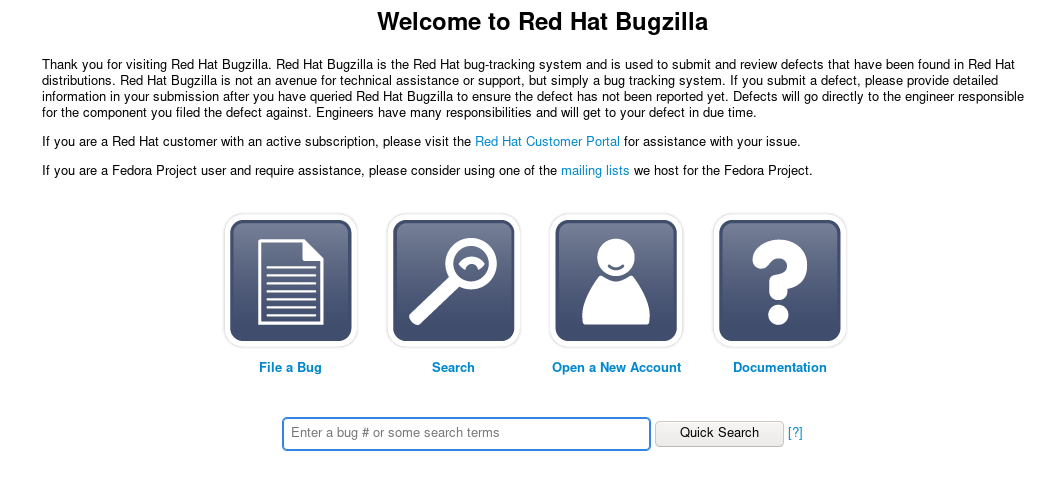
\includegraphics[width=10cm]{images/bz_new.png}
\end{frame}

\begin{frame}{Logged into Bugzilla}
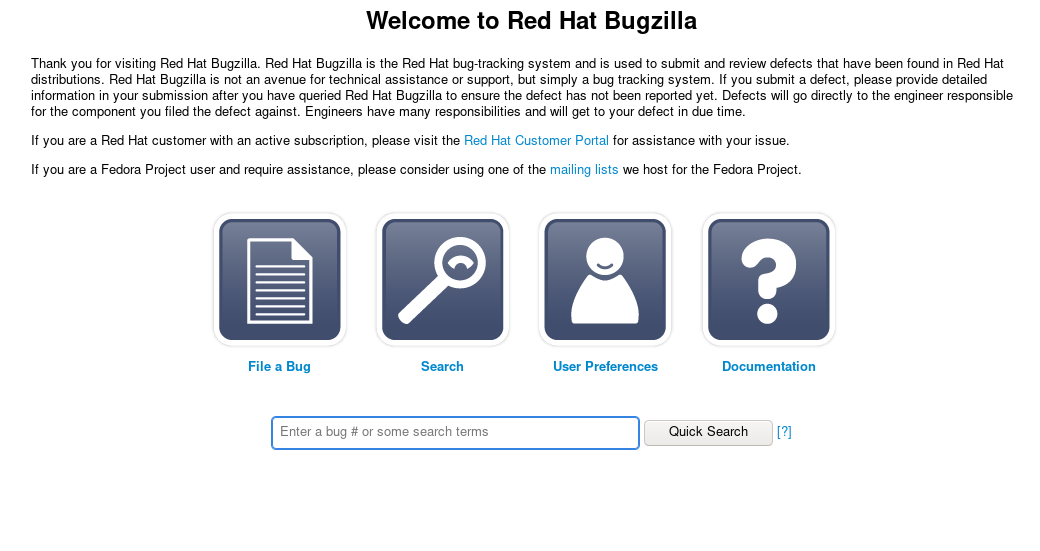
\includegraphics[width=10cm]{images/bz_logged.png}
\end{frame}

\begin{frame}{Classify the bug}
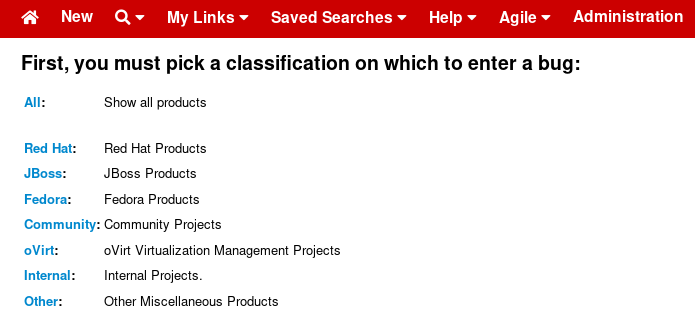
\includegraphics[width=10cm]{images/bz_classification.png}
\end{frame}

\begin{frame}{Choose the correct product}
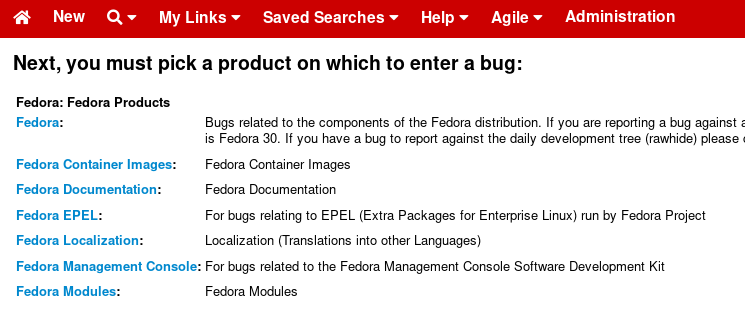
\includegraphics[width=10cm]{images/bz_product.png}
\end{frame}

\begin{frame}{File the bug (part 1)}
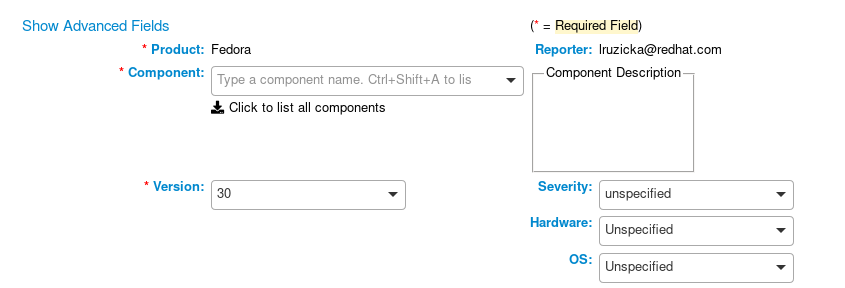
\includegraphics[width=10cm]{images/bz_header.png}
\end{frame}

\begin{frame}{File the bug (part 2)}
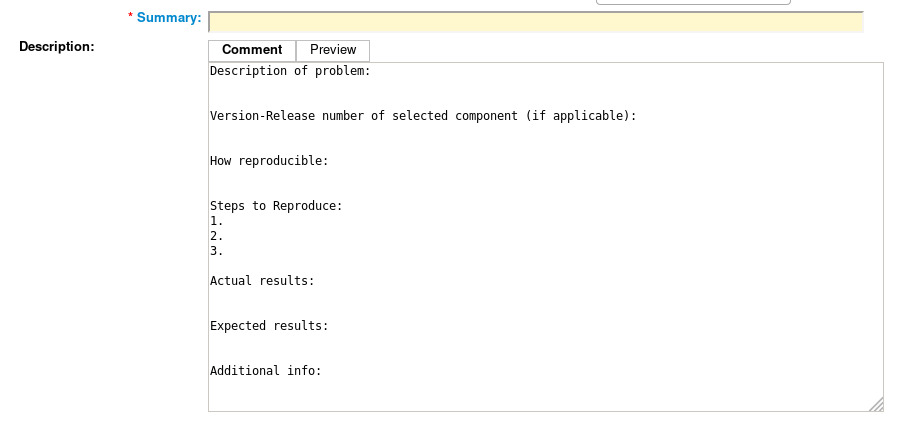
\includegraphics[width=10cm]{images/bz_description.png}
\end{frame}

\begin{frame}{Description of problem}
\begin{itemize}
	\item What is the problem?
	\item When does it appear?
	\item How much does it affect work?
	\item Why is it a problem?
	\item others
\end{itemize}
\end{frame}

\begin{frame}[fragile]{Version of selected component}
Provide the version number of the problematic components and also of the affected components.
\begin{itemize}
	\item {\color{blue}\textbf{About}} menu in GUI
	\item {\color{blue}\texttt{-v}} or {\color{blue}{\verb|--version|}} option on CLI (or \texttt{man})
	\item {\color{blue}\texttt{rpm -q}} for installed packages
	\item {\color{blue}\texttt{dnf info}} for installed and available packages
\end{itemize}
\end{frame}

\begin{frame}{How reproducible}
\begin{itemize}
	\item Always
	\item Sometimes -- specify when exactly
	\item Under certain conditions -- describe them
	\item Heisenbug 
\end{itemize}
\end{frame}

\begin{frame}{Steps to reproduce}
Procedure that leads to reproducing the bug.
\begin{itemize}
	\item One activity in one step.
	\item Do not skip steps, even if you think the step is obvious.
	\item Pay attention to details.
	\item Be exact.
\end{itemize}
Others want to see that bug, too. 
\end{frame}

\begin{frame}{Results}
\begin{description}
	\item[Actual] -- what is the result of the current behaviour
	\item[Expected] -- how you think the system should behave
\end{description}
\end{frame}

\begin{frame}{File the bug (part 3)}

\includegraphics[width=10cm]{images/bz_footer.png}
\end{frame}

\begin{frame}{No clue about anything?}

{\Large File the bug anyway!}
\end{frame}

\begin{frame}{Q\&A}

{\Large Question time.}
\end{frame}

\begin{frame}{End}

{\Large Thank you for coming!}
\end{frame}

\end{document}